\documentclass[11pt,a4paper,oneside]{report}             % Single-side
%\documentclass[11pt,a4paper,twoside,openright]{report}  % Duplex

\usepackage{ifxetex}
\ifxetex
  \usepackage{fontspec}
\else
  \usepackage[T1]{fontenc}
  \usepackage[utf8]{inputenc}
  \usepackage{lmodern}
\fi

\usepackage[english,magyar]{babel} % Alapértelmezés szerint utoljára definiált nyelv lesz aktív, de később külön beállítjuk az aktív nyelvet.

\usepackage{cmap}
\usepackage{amsfonts,amsmath,amssymb} % Mathematical symbols.
\usepackage[ruled,boxed,resetcount,linesnumbered]{algorithm2e} % For pseudocodes.
\usepackage{booktabs} % For publication quality tables for LaTeX
\usepackage{graphicx}


%\usepackage{fancyhdr}
%\usepackage{lastpage}

\usepackage{anysize}
\usepackage{sectsty}
\usepackage{setspace}  % Ettol a tablazatok, abrak, labjegyzetek maradnak 1-es sorkozzel!

\usepackage{hyperref} % For hyperlinks in the generated document. 
\usepackage{color}
\usepackage{listings} % For source code snippets.

\usepackage[amsmath,thmmarks]{ntheorem} % Theorem-like environments.

\usepackage[hang]{caption}





%%--------------------------------------------------------------------------------------
% Elnevezések
%--------------------------------------------------------------------------------------
\newcommand{\dolgozatnyelve}{\selectlanguage{magyar}}

\newcommand{\bme}{Budapesti Műszaki és Gazdaságtudományi Egyetem}
\newcommand{\vik}{Villamosmérnöki és Informatikai Kar}

\newcommand{\bmemit}{Méréstechnika és Információs Rendszerek Tanszék}

\newcommand{\keszitette}{Készítette}
\newcommand{\konzulens}{Konzulens}

\newcommand{\bsc}{Szakdolgozat}
\newcommand{\msc}{Diplomaterv}

\newcommand{\pelda}{Példa}
\newcommand{\definicio}{Definíció}
\newcommand{\tetel}{Tétel}

\newcommand{\bevezeto}{Bevezető}
\newcommand{\koszonetnyilvanitas}{Köszönetnyilvánítás}
\newcommand{\abrakjegyzeke}{Ábrák jegyzéke}
\newcommand{\tablazatokjegyzeke}{Táblázatok jegyzéke}
\newcommand{\irodalomjegyzek}{Irodalomjegyzék}
\newcommand{\fuggelek}{Függelék}

\newcommand{\szerzo}{\vikszerzoVezeteknev{} \vikszerzoKeresztnev}


\newcommand{\englishParagraph}{
	\setlength{\parindent}{0em} % angol nyelvű dokumentumokban jellemző
	\setlength{\parskip}{0.5em} % angol nyelvű dokumentumokban jellemző
	\nonfrenchspacing
}

\newcommand{\hungarianParagraph}{
	\setlength{\parindent}{2em} % angol nyelvű dokumentumokban jellemző
	\setlength{\parskip}{0em}   % angol nyelvű dokumentumokban jellemző
	\frenchspacing
}

\newcommand{\defaultParagraph}{
	\hungarianParagraph
}

\bibliographystyle{huplain}
  % Beállítások magyar nyelvű dolgozathoz
%--------------------------------------------------------------------------------------
% Elnevezések
%--------------------------------------------------------------------------------------
\newcommand{\dolgozatnyelve}{\selectlanguage{english}}

\newcommand{\bme}{Budapest University of Technology and Economics}
\newcommand{\vik}{Faculty of Electrical Engineering and Informatics}

\newcommand{\bmemit}{Department of Measurement and Information Systems}

\newcommand{\keszitette}{Author}
\newcommand{\konzulens}{Advisor}

\newcommand{\bsc}{Bachelor's Thesis}
\newcommand{\msc}{Master's Thesis}

\newcommand{\pelda}{Example}
\newcommand{\definicio}{Definition}
\newcommand{\tetel}{Theorem}

\newcommand{\bevezeto}{Introduction}
\newcommand{\koszonetnyilvanitas}{Acknowledgements}
\newcommand{\abrakjegyzeke}{List of Figures}
\newcommand{\tablazatokjegyzeke}{List of Tables}
\newcommand{\irodalomjegyzek}{Bibliography}
\newcommand{\fuggelek}{Appendix}

\newcommand{\szerzo}{\vikszerzoKeresztnev{} \vikszerzoVezeteknev}

\newcommand{\englishParagraph}{
	\setlength{\parindent}{0em} % angol nyelvű dokumentumokban jellemző
	\setlength{\parskip}{0.5em} % angol nyelvű dokumentumokban jellemző
	\nonfrenchspacing
	\renewcommand{\figureautorefname}{Figure}
	\renewcommand{\tableautorefname}{Table}
	\renewcommand{\partautorefname}{Part}
	\renewcommand{\chapterautorefname}{Chapter}
	\renewcommand{\sectionautorefname}{Section}
	\renewcommand{\subsectionautorefname}{Section}
	\renewcommand{\subsubsectionautorefname}{Section}
}


\newcommand{\hungarianParagraph}{
	\setlength{\parindent}{2em} % angol nyelvű dokumentumokban jellemző
	\setlength{\parskip}{0em}   % angol nyelvű dokumentumokban jellemző
	\frenchspacing
}

\newcommand{\defaultParagraph}{
	\englishParagraph
}

\newcommand{\ie}{i.e.\@\xspace}
\newcommand{\Ie}{I.e.\@\xspace}
\newcommand{\eg}{e.g.\@\xspace}
\newcommand{\Eg}{E.g.\@\xspace}
\newcommand{\etal}{et al.\@\xspace}
\newcommand{\etc}{etc.\@\xspace}

\bibliographystyle{plain}
 % Settings for English documents

%--------------------------------------------------------------------------------------
% Main variables


%--------------------------------------------------------------------------------------
\newcommand{\vikszerzoVezeteknev}{Kővári}
\newcommand{\vikszerzoKeresztnev}{Zsolt}
\newcommand{\vikkonzulensA}{Gábor Szárnyas} % Első konzulens neve
\newcommand{\vikkonzulensB}{Dr. István Ráth} % Második konzulens neve; hagyd üresen, ha egy konzulensed van.
\newcommand{\vikcim}{Performance Analysis of Graph Queries} % Cím
\newcommand{\viktanszek}{\bmemit} % Tanszék
\newcommand{\vikdoktipus}{\msc} % Dokumentum típusa (diplomaterv, szakdolgozat, TDK-dolgozat, stb.)

%--------------------------------------------------------------------------------------
% TDK-specifikus változók
%--------------------------------------------------------------------------------------
\newcommand{\tdkszerzoB}{} % Második szerző neve; hagyd üresen, ha egyedül í­rtad a TDK-t.
\newcommand{\tdkev}{2015} % A dolgozat írásának éve (pl. "2014") (Ez OTDK-nál eltérhet az aktuális évtől.)

% További adatok az OTDK címlaphoz (BME-s TDK-hoz nem kell kitölteni)
\newcommand{\tdkevfolyamA}{IV} % Első szerző évfolyama, római számmal (pl. IV).
\newcommand{\tdkevfolyamB}{III} % Második szerző évfolyama, római számmal (pl. III).
\newcommand{\tdkkonzulensbeosztasA}{egyetemi tanár} % Első konzulens beosztása (pl. egyetemi docens)
\newcommand{\tdkkonzulensbeosztasB}{doktorandusz} % Második konzulens beosztása (pl. egyetemi docens)
\newcommand{\szerzoMeta}{\vikszerzoVezeteknev{} \vikszerzoKeresztnev} % egy szerző esetén
%\newcommand{\szerzoMeta}{\vikszerzoVezeteknev{} \vikszerzoKeresztnev, \tdkszerzoB} % két szerző esetén

%--------------------------------------------------------------------------------------
% Page layout setup
%--------------------------------------------------------------------------------------
% we need to redefine the pagestyle plain
% another possibility is to use the body of this command without \fancypagestyle
% and use \pagestyle{fancy} but in that case the special pages
% (like the ToC, the References, and the Chapter pages)remain in plane style

\pagestyle{plain}
\marginsize{35mm}{25mm}{15mm}{15mm}

\setcounter{secnumdepth}{0}
\sectionfont{\large\upshape\bfseries}
\setcounter{secnumdepth}{2}

\sloppy % Margón túllógó sorok tiltása.
\widowpenalty=10000 \clubpenalty=10000 %A fattyú- és árvasorok elkerülése
\def\hyph{-\penalty0\hskip0pt\relax} % Kötőjeles szavak elválasztásának engedélyezése


%--------------------------------------------------------------------------------------
% Setup hyperref package
%--------------------------------------------------------------------------------------
\hypersetup{
    bookmarks=true,            % show bookmarks bar?
    unicode=false,              % non-Latin characters in Acrobat's bookmarks
    pdftitle={\vikcim},        % title
    pdfauthor={\szerzoMeta},    % author
    pdfsubject={\vikdoktipus}, % subject of the document
    pdfcreator={\szerzoMeta},   % creator of the document
    pdfproducer={},    % producer of the document
    pdfkeywords={},    % list of keywords (separate then by comma)
    pdfnewwindow=true,         % links in new window
    colorlinks=true,           % false: boxed links; true: colored links
    linkcolor=black,           % color of internal links
    citecolor=black,           % color of links to bibliography
    filecolor=black,           % color of file links
    urlcolor=black             % color of external links
}


%--------------------------------------------------------------------------------------
% Set up listings
%--------------------------------------------------------------------------------------
\definecolor{lightgray}{rgb}{0.95,0.95,0.95}
\lstset{
	basicstyle=\scriptsize\ttfamily, % print whole listing small
	keywordstyle=\color{black}\bfseries, % bold black keywords
	identifierstyle=, % nothing happens
	commentstyle=\color{green}, % green comments
	stringstyle=\scriptsize,
	showstringspaces=false, % no special string spaces
	aboveskip=3pt,
	belowskip=3pt,
	backgroundcolor=\color{lightgray},
	columns=flexible,
	keepspaces=true,
	escapeinside={(*@}{@*)},
	literate=*
		{á}{{\'a}}1	{é}{{\'e}}1	{í}{{\'i}}1	{ó}{{\'o}}1	{ö}{{\"o}}1	{ő}{{\H{o}}}1	{ú}{{\'u}}1	{ü}{{\"u}}1	{ű}{{\H{u}}}1
		{Á}{{\'A}}1	{É}{{\'E}}1	{Í}{{\'I}}1	{Ó}{{\'O}}1	{Ö}{{\"O}}1	{Ő}{{\H{O}}}1	{Ú}{{\'U}}1	{Ü}{{\"U}}1	{Ű}{{\H{U}}}1
} 	
\def\lstlistingname{lista}	


%--------------------------------------------------------------------------------------
% Set up theorem-like environments
%--------------------------------------------------------------------------------------
% Using ntheorem package -- see http://www.math.washington.edu/tex-archive/macros/latex/contrib/ntheorem/ntheorem.pdf

\theoremstyle{plain}
\theoremseparator{.}
\newtheorem{example}{\pelda}

\theoremseparator{.}
%\theoremprework{\bigskip\hrule\medskip}
%\theorempostwork{\hrule\bigskip}
\theorembodyfont{\upshape}
\theoremsymbol{{\large \ensuremath{\centerdot}}}
\newtheorem{definition}{\definicio}

\theoremseparator{.}
%\theoremprework{\bigskip\hrule\medskip}
%\theorempostwork{\hrule\bigskip}
\newtheorem{theorem}{\tetel}


%--------------------------------------------------------------------------------------
% Some new commands and declarations
%--------------------------------------------------------------------------------------
\newcommand{\code}[1]{{\upshape\ttfamily\scriptsize\indent #1}}
\newcommand{\doi}[1]{DOI: \href{http://dx.doi.org/\detokenize{#1}}{\raggedright{\texttt{\detokenize{#1}}}}} % A hivatkozások közt így könnyebb DOI-t megadni.

\newcommand{\CC}{C\nolinebreak\hspace{-.05em}\raisebox{.4ex}{\tiny\bf +}\nolinebreak\hspace{-.10em}\raisebox{.4ex}{\tiny\bf +}}

\DeclareMathOperator*{\argmax}{arg\,max}
%\DeclareMathOperator*[1]{\floor}{arg\,max}
\DeclareMathOperator{\sign}{sgn}
\DeclareMathOperator{\rot}{rot}


%--------------------------------------------------------------------------------------
% Setup captions
%--------------------------------------------------------------------------------------
\captionsetup[figure]{
	width=.75\textwidth,
	aboveskip=10pt}

\renewcommand{\captionlabelfont}{\bf}
%\renewcommand{\captionfont}{\footnotesize\it}


%--------------------------------------------------------------------------------------
% Redefine reference style
%--------------------------------------------------------------------------------------
\newcommand{\figref}[1]{\ref{fig:#1}.}
\renewcommand{\eqref}[1]{(\ref{eq:#1})}
\newcommand{\listref}[1]{\ref{listing:#1}.}
\newcommand{\sectref}[1]{\ref{sect:#1}}
\newcommand{\tabref}[1]{\ref{tab:#1}.}


%--------------------------------------------------------------------------------------
% Hyphenation exceptions
%--------------------------------------------------------------------------------------
\hyphenation{Shakes-peare Mar-seilles ár-víz-tű-rő tü-kör-fú-ró-gép}


\author{\vikszerzo}
\title{\viktitle}


%--------------------------------------------------------------------------------------
% Table of contents and the main text
%--------------------------------------------------------------------------------------
\begin{document}



%~~~~~~~~~~~~~~~~~~~~~~~~~~~~~~~~~~~~~~~~~~~~~~~~~~~~~~~~~~~~~~~~~~~~~~~~~~~~~~~~~~~~~~
%\pagenumbering{gobble}
\dolgozatnyelve
\hungarianParagraph
\singlespacing
%--------------------------------------------------------------------------------------
% Rovid formai es tartalmi tajekoztato
%--------------------------------------------------------------------------------------

\footnotesize
\begin{center}
\large

\end{center}



%%--------------------------------------------------------------------------------------
% Feladatkiiras (a tanszeken atveheto, kinyomtatott valtozat)
%--------------------------------------------------------------------------------------
\clearpage
\begin{center}
\large
\textbf{FELADATKIÍRÁS}\\
\end{center}

A feladatkiírást a tanszéki adminisztrációban lehet átvenni, és a leadott munkába eredeti, tanszéki pecséttel ellátott és a tanszékvezető által aláírt lapot kell belefűzni (ezen oldal \emph{helyett}, ez az oldal csak útmutatás). Az elektronikusan feltöltött dolgozatban már nem kell beleszerkeszteni ezt a feladatkiírást.


\pagenumbering{gobble}
\dolgozatnyelve
\englishParagraph
\singlespacing
%%--------------------------------------------------------------------------------------
% Feladatkiiras (a tanszeken atveheto, kinyomtatott valtozat)
%--------------------------------------------------------------------------------------
\clearpage
\begin{center}
\large
\textbf{FELADATKIÍRÁS}\\
\end{center}

A feladatkiírást a tanszéki adminisztrációban lehet átvenni, és a leadott munkába eredeti, tanszéki pecséttel ellátott és a tanszékvezető által aláírt lapot kell belefűzni (ezen oldal \emph{helyett}, ez az oldal csak útmutatás). Az elektronikusan feltöltött dolgozatban már nem kell beleszerkeszteni ezt a feladatkiírást.

\onehalfspacing
\defaultParagraph



%~~~~~~~~~~~~~~~~~~~~~~~~~~~~~~~~~~~~~~~~~~~~~~~~~~~~~~~~~~~~~~~~~~~~~~~~~~~~~~~~~~~~~~
	%%--------------------------------------------------------------------------------------
%	The title page
%--------------------------------------------------------------------------------------
\begin{titlepage}
\begin{center}

\includegraphics[width=60mm,keepaspectratio]{figures/bme_logo.pdf}\\
\vspace{0.3cm}
\textbf{\bme}\\
\textmd{\vik}\\
\textmd{\viktanszek}\\[5cm]

\vspace{0.4cm}
{\huge \bfseries \vikcim}\\[0.8cm]
\vspace{0.5cm}
\textsc{\Large \vikdoktipus}\\[4cm]

{
	\renewcommand{\arraystretch}{0.85}
	\begin{tabular}{cc}
	 \makebox[7cm]{\emph{\keszitette}} & \makebox[7cm]{\emph{\konzulens}} \\ \noalign{\smallskip}
	 \makebox[7cm]{\szerzo} & \makebox[7cm]{\vikkonzulensA} \\
	  & \makebox[7cm]{\vikkonzulensB} \\
	\end{tabular}
}

\vfill
{\large \today}
\end{center}
\end{titlepage}


		   % Szakdolgozat/Diplomaterv címlap
	%% TDK címlap
\begin{titlepage}
  \begin{center}  
  
\includegraphics[width=7cm]{./figures/bme_logo.pdf}
  \vspace{0.3cm}
  
  \bme \\
  \vik \\
  \viktanszek \\
  \vspace{5cm}
  
  \huge {\vikcim}
  \vspace{1.5cm}
  
  \large {\textbf{\vikdoktipus}}
  \vfill
    
  {\Large 
  	\keszitette: \\ \vspace{0.3cm}
  	\szerzo \\
  	\vspace{1.5cm}
  	\konzulens: \\ \vspace{0.3cm}
  	\vikkonzulensA \\
  	\vikkonzulensB \\
  }
  
  \vspace{2cm}
  \large {\tdkev.}
 \end{center}
\end{titlepage}
%% Címlap vége	% TDK címlap
	%%% OTDK külső címlap
\begin{titlepage}
  	$\;$ 
	\vspace{5cm}
	
	\begin{center}
	\Huge
	\textbf{TDK-dolgozat}\let\thefootnote\relax\footnote{A dolgozat bemutatását a XXXXXXXXX  ``Lorem ipsum dolor sit amet'' című program támogatta.}
	\end{center}
	
	\vspace{13cm}
	
	\Large
	\hspace{8cm} \szerzo
	
	\hspace{8cm} \tdkszerzoB
	
	\hspace{8cm} \tdkev.
\end{titlepage}

\newpage
\thispagestyle{empty}


%% OTDK belső címlap
\begin{titlepage}
  \begin{center}  
  
\includegraphics[width=7cm]{./figures/bme_logo.pdf}
  \vspace{0.3cm}
  
  \bme \\
  \vik \\
  \viktanszek \\
  \vspace{3.5cm}
  
  \huge {\vikcim}
  \vspace{1.5cm}
  
  \large {\textbf{\vikdoktipus}}
  \vfill
    
  {\Large 
  	{\large \keszitette:} \\ \vspace{0.2cm}
  	\szerzo \\ \tdkevfolyamA. évfolyam \\
	\vspace{0.5cm}
	\tdkszerzoB \\ \tdkevfolyamB. évfolyam \\
  	\vspace{1.5cm}
  	{\large \konzulens:} \\ \vspace{0.2cm}
  	\vikkonzulensA,\\ \tdkkonzulensbeosztasA \\
  	\vspace{0.5cm}
  	\vikkonzulensB,\\ \tdkkonzulensbeosztasB \\
  }
  
  \vspace{2cm}
  \large {\tdkev.}
  
 \end{center}
\end{titlepage}   % OTDK címlap
 

% Table of Contents
%~~~~~~~~~~~~~~~~~~~~~~~~~~~~~~~~~~~~~~~~~~~~~~~~~~~~~~~~~~~~~~~~~~~~~~~~~~~~~~~~~~~~~~
	\tableofcontents\vfill


% Declaration and Abstract
%~~~~~~~~~~~~~~~~~~~~~~~~~~~~~~~~~~~~~~~~~~~~~~~~~~~~~~~~~~~~~~~~~~~~~~~~~~~~~~~~~~~~~~
	\pagenumbering{roman}
\setcounter{page}{1}

\selectlanguage{magyar}
%\hungarianParagraph

\englishParagraph
%----------------------------------------------------------------------------
% Abstract in Hungarian
%----------------------------------------------------------------------------
\chapter*{Kivonat}\addcontentsline{toc}{chapter}{Kivonat}

A gráf alapú adatmodellező, illetve adatbázis-kezelő keretrendszerek esetén kulcsfontosságú a minél nagyobb teljesítmény, illetve rövidebb válaszidő biztosítása, különösen az olyan alkalmazási területeken, ahol egyszerre több, strukturálisan összetett lekérdezést kell újra és újra kiértékelni egy folyamatosan változó (gráf)adatstruktúra felett. A modern, relációs adatmodellt elvető NoSQL technológiák terjedésével egyre nagyobb figyelmet kap az ilyen rendszerek teljesítőképessége és skálázhatósága, így az utóbbi években több olyan benchmark is megjelent, melynek fő célja az ilyen rendszerek teljesítőképességének, különösen a lekérdezések skálázhatóságának szisztematikus kiértékelése. 

A legtöbb mérési keretrendszer számításba vesz bemenet és teljesítmény leíró metrikákat, mint például a gráf csomópontjainak száma vagy a lekérdezések válaszideje, ugyanakkor nagyon nehéz az eredmények összehasonlítása, mert a méréshez használt bemenetek (gráfok, lekérdezések komplexitása, illetve a gráfon a mérés során végrehajtott változtatások jellege, összességében a \emph{terhelési profil}) igen nagy méret- és tulajdonságbeli eltéréseket mutatnak - ezekről pedig megelőző kutatási eredmények kimutatták, hogy jelentős és változó mértékben befolyásolhatják az egyes eszközök viselkedését, teljesítménykarakterisztikáját.
% Azonban, ezen keretrendszerek nem veszik figyelembe a gráf belső hálózatán végbemenő változásokat, és kizárólag egy struktúrájú gráfra koncentrálnak. 

A jelen dolgozat elsődleges célja, hogy - korábbi kutatásokat folytatva - kidolgozzon egy olyan mérési módszertant és hozzá kapcsolódó keretrendszert, amelynek segítségével a gráf alapú adatbázis-kezelő rendszerek teljesítménybeli összehasonlítása szisztematikusan és reprodukálhatóan hajtható végre. Fő eredményként a teljesítménymérés céljára különböző gráf topológiákat javasolunk, amelyek jellemzésére gráfmetrikákat definiálunk. A metrikák segítségével jellemezhető az egyes mérések nehézsége, illetve bizonyos eszközök esetén kapcsolatot is találhatunk a gráfokat jellemző metrikák és a lekérdezések futásidői között. A módszertan és a keretrendszer képességeinek bemutatására a dolgozat bemutat egy komplex esettanulmányt, mely magába foglalja számos kísérlet automatizált elvégzését és magasszintű statisztikai analízis eszközökkel támogatott kiértékelését is.

%, így metrikáink később felhasználhatóak a gráflekérdezések optimalizálása - jelenleg még nagyon kiforratlan - területén. 



\vfill
\selectlanguage{english}
\englishParagraph


%----------------------------------------------------------------------------
% Abstract in English
%----------------------------------------------------------------------------
\chapter*{Abstract}\addcontentsline{toc}{chapter}{Abstract}
Achieving high-performance query evaluation represents a crucial problem in modern graph-based database systems. The response time of the query evaluation on a graph is affected by the complexity of the particular query and the underlying network structure of the graph. 

Several state-of-the-art benchmark frameworks exist that assess the performance and correctness of query evaluations as they create real world-like workloads and define suites of systematic queries. However, these benchmark frameworks rely on only one particular type of network and they do not concentrate on a significant alteration of the underlying graph. Although most of them define metrics for characterizing the specific aspects of performance (response time, query evaluations per hour, etc.), most of them lack such comprehensive metrics for the queries and the graph.
As a consequence, they cannot determine the correlations between workload and performance.

%Due to the absence of metrics, it is difficult to give a precise characterization of the complexity for various benchmarks. Hence, it is difficult %to compare the benchmarks and the published results to each other.

In order to provide solid foundations to characterize the complexity of graph benchmarks, we elaborate a benchmark framework for graph-based database systems.

We use various graph metrics to describe the structure of the graph %create regression models to determine the relationships quantitatively.
and use a varied set of graph topologies for benchmarking. This will allow us to perform in-depth analysis on the relationships between the structure of the graph in the database and the performance of the query evaluations. These results can be used to obtain advanced heuristics for the optimization of graph query engines. While the optimization of relational databases has well-known techniques documented by a wide literature, the problem for graph query engines is yet be discussed thoroughly.




%The performance of query evaluations depends on the topology of the model, and the complexity of the particular query. Our primary goal is that --- %by defining model and query-related quantitative metrics ---  to find a considerable connection between metrics and the performance, and thus, be %able to predict the query evaluation time.

%Based on the metrics and their effect to the performance, we are able to make decisions in design to achieve on the optimal performance. %Furthermore, this knowledge can be utilized in the area of real-time query optimization engines as well.

%We investigate various NoSQL database systems via regression analysis in order to find different model-related metrics that are suited to %characterize their performance appropriately. Based on a real model, we generate graphs with various topologies and distributions to find metrics %from different aspects.

%Furthermore, we explore that whether an arbitrarily structured model's performance is predictable via our regression analysis, and also predict %which database system from our scope can be associated to the model in order to achieve an optimal performance.

%Finally, being motivated by the real-time optimization engines, we search answers whether by reducing the cost of metric calculations, an arbitrary %model's performance is still predictable.


\vfill
\dolgozatnyelve
\defaultParagraph

\newcounter{romanPage}
\setcounter{romanPage}{\value{page}}
\stepcounter{romanPage}	  %TODO Összefoglaló -- TDK és OTDK esetén nem kötelező


% The main part of the thesis
%~~~~~~~~~~~~~~~~~~~~~~~~~~~~~~~~~~~~~~~~~~~~~~~~~~~~~~~~~~~~~~~~~~~~~~~~~~~~~~~~~~~~~~
\pagenumbering{arabic}


	%----------------------------------------------------------------------------
\chapter*{Introduction}\addcontentsline{toc}{chapter}{\bevezeto}
%----------------------------------------------------------------------------

% Queries in MDE: scalability challenge
Nowadays, model-driven software engineering (MDSE) plays an important role in the development processes of critical embedded systems. Advanced modeling tools provide support for a wide range of development tasks such as requirements and traceability management, system modeling, early design validation, automated code generation, model-based testing and other validation and verification tasks. With the dramatic increase in complexity that is also affecting critical embedded systems in recent years, modeling toolchains are facing scalability challenges as the size of design models constantly increases, and automated tool features become more sophisticated.

% Techniques to achieve scalability
A key factor in the scalability of MDE toolchains is the performance of model representation~\cite{GrandChallengeScalability}, which is, in turn, determined by the characteristics of persistence, query evaluation and model manipulation operations. Traditionally, modeling tools built on state-of-the-art frameworks such as the Eclipse Modeling Framework (EMF~\cite{EMF}) have relied on an in-memory object model backed by an XML serialization. More recently, \emph{model repositories} (such as CDO~\cite{CDO} or Morsa~\cite{COLLAB:MORSA}) have emerged that aim to tackle scalability issues by making use of advances in object persistence technology. As the majority of model-based tools uses a graph-oriented data model, recent results of the NoSQL and Linked Data movement~\cite{neo4j,openvirtuoso,sesame} are straightforward candidates for adaptation to MDE purposes. 

\emph{Model queries} support several essential scenarios including model validation, model transformations, model synchronization, view maintenance and model execution. As a consequence, many scalability issues can be addressed by improving query performance. This led to the development of several model indexing and query evaluation engines (such as Eclipse OCL~\cite{EclipseOCL}, EMF Query~\cite{EMF:ModelQuery}, complementary approaches that translate model queries into lower level queries that can be executed on the (relational) back-end~\cite{scheidgen2012automated}). 
There are also several approaches (such as \mbox{\textsc{EMF-IncQuery}}~\cite{models10} and the Impact Analyzer of Eclipse OCL~\cite{EclipseOCL}) to support the \emph{incremental evaluation} of model queries, which reduces query response time by limiting the impact of model modifications to query result calculation.

% Benchmarks
For tool engineers, \emph{benchmarks} may provide guidance on picking the right technology for building a new tool architecture to fulfill increasing scalability requirements. Due to their central role in data-intensive applications, the performance of persistence technologies has been evaluated by many benchmarks~\cite{BSBM,SP2Bench} % TODO cite
that focus on throughput and response time measurements, and investigate scalability in terms of the size of the data set and the number of transactions. In addition to these traditional scalability aspects, the semantic web community has investigated the scalability of semantic graph databases (RDF triple stores). These benchmarks rely on graph queries over a structurally richer data set and also investigate the effects of advanced semantic technologies such as inference. Up to now, the most complex benchmarking workloads have been investigated by the academic and industrial MDE tool building community in transformation tool contests~\cite{TTC}, which feature synthetic model transformation case studies inspired by real-world applications.

% Challenges: lack of predictability, and generalizability to actual MDSE workloads
% key differences
Despite all these efforts, \emph{making a well-founded technological choice} based on existing benchmarking results \emph{remains a tough challenge}. First, MDE tools have very specific \emph{workloads} (both in terms of model structure and transaction complexity) \emph{that are different} in key aspects compared to traditional RDBMS and newer graph persistence benchmarks. MDE tools rely on much more complex queries and their performance is dominated by response time and re-evaluation time rather than throughput. Additionally, RDBMS and semantic technologies have key conceptual differences that require mapping layers which might have adverse and unpredictable effects on real life performance.
The generalizability of benchmark results is further limited by the \emph{scarcity of relevant metrics} that could be used to assess an engineering problem and predict which technology would be best suited. Existing metrics emphasize a single aspect of the problem (most typically model size), while internal metrics (used by e.g. optimizing query evaluation engines or pattern matchers inside GT tools, for estimating query evaluation difficulty) are either not documented well or not accessible in a reusable way.


In this paper, we aim to address these challenges by \emph{assessing existing metrics, along with newly proposed ones}. These metrics take instance model characteristics, static query characteristics and their combination into account. Based on our real-life experiences with tools and models, we \emph{outline a benchmark} that uses model validation as its core scenario, thus focusing on model loading and model validation workloads. Guidelines are provided on the generation of instance models and queries, on which we evaluated the metrics and executed the benchmark using three, characteristically different graph query tools. In order to identify which metrics provide reliable performance prediction for a given workload and tool category, we \emph{calculate the correlation with significance values} between execution times and metrics.

% % proposal: metrics for estimation, benchmark for differentiation 
% In this paper, we aim to address these challenges by \emph{assessing (existing and novel) metrics} that take instance model characteristics, static query characteristics and their combination %of both query and instance model characteristics 
% into account. 
% By providing guidelines on instance model generation and case study fine tuning to achieve result dispersion (to provide differentiation between various technologies), we outline a benchmark that uses model validation as the core scenario.
% Our experimental measurements evaluate the metrics over the test set of our benchmark over  three characteristically different classes of query technologies. We calculate the correlation of the predictions provided by the metrics with the measurement data to highlight which metrics provide reliable prediction for a certain query technology.
% %with results to identity those metrics that can reliably predict application performance.

% Structure
The rest of the paper is structured as follows. 
\autoref{sec:background} overviews the most important concepts of modeling languages and model queries, and 
\autoref{sec:relwork} discusses benchmarking and metrics related work.
\autoref{sec:benchmark} presents our analysis of existing benchmarks and proposes new metrics and benchmarks, with their evaluation presented in \autoref{sec:eval}.
\autoref{sec:conclusion} outlines directions for future work and concludes the paper.

	
\chapter{Background}\label{chapter:background}

\section{The Trainbenchmark Framework}\label{section:trainbenchmark}

In the following section, we introduce Train Benchmark, a framework on which our search is based to find empirical connections between
different models and the related evaluated queries in order to estimate query evaluation time. The next few sections explain the main goal of the framework and represent the most important components in the system on which we will concentrate in the later chapters. Apart from these, we also allude some obsolete parts of the framework and emphasize their disadvantages in order to make understandable the main motivation of design decisions that resulted in some considerable modifications in the system.

\subsection{Main Concepts}

The basic idea and implementation of the Train Benchmark framework was introduced by the Fault Tolerant Systems Research Group in the Budapest
University of Technology and Economics. The implementation is written in Java programming language. Basically, Train Benchmark focuses on the performance of model validations in which the goal is to find those elements from a model that violate the well-formedness constraints. \footnote{A well-formedness constraint is defined on the model and it is considered as a definition of a particular rule belonging to the elements in the model. For example, a constraint can order the cardinality of the elements, or it can define maximum bounds for attributes, etc.} The model validations are accomplished by different databases systems, where the validation appears as a query evaluation, and the measured performance by the system is the evaluation time of the particular query. For the sake of clarity, Figure 1 represents the main steps of the framework's workflow.

The first step is the model generation and the definition of the well-formedness constraints. The Train Benchmark framework uses artificially generated graph-based models with the same domain, it and describes different constraints on them. Since the main goal is to assess model validations, a perfectly valid model generation is not advisable, thus, some fault injections are required during the generation phase, when a subset of the elements (typically 2-5\%) violates the well-formedness constraints. 

The second step is loading the model to the database systems. Subsequently, the generated model is already accessible from the database's repository, and stored in their own format. The next phase is the model validation itself, when a validation---defined in the particular database's query language---is evaluated and its result set includes those erroneous elements from the model that violate the well-formedness constraints. Thus, a model validation occurs and the required time of the query evaluation is measured as well. The validation time will play the most important indicator in the performance comparison among different databases.
 %todo insert validation pic
To summarize, the Train Benchmark framework uses artificially generated graph-based models to investigate the model validation times and thus, the performance of different database systems. In the following, we introduce the domain of the model and its typical characteristics, furthermore, we also define the scope of the framework, as represent the used databases.

\subsection{The Metamodel} \label{section:metamodel}

As we referred in \ref{section:trainbenchmark}, there were some components in the Train Benchmark framework that needed to reconstruct in order to obtain precise statistical analysis of model and query metric relationships. One of them was the original domain of the framework, the metamodel. However, (i) to understand the motivations of changing the domain entirely, (ii) to see the contrast between the two of them, and (iii) also recognize the possible virtues that we obtained by introducing a now domain, it is important to represent the original domain in this section.

At first, let define the basic related concepts.

\paragraph{Metamodel and Instance Model}

A metamodel is considered as an abstract model of another model, where the prior---the metamodel---defines the available elements and their cardinalities, additionally, it order rules, constraints on the elements which are used in the latter. Then, a concrete instance of a metamodel is called instance model which can use those elements that are defined in the metamodel, and it must also obey the specified rules and constraints, otherwise, it is considered as an invalid model which violates the constraints in the metamodel.

The domain, or the metamodel\footnote{We use the concepts of domains and metamodels as synonyms in this paper.} of Train Benchmark is depicted in Figure 2, and it is related to a railway network (here comes the name of the benchmark framework). A train route is defined by a sequence of sensors. Sensors are associated with track elements which are either segments (with a specific length) or
switches. A route follows certain switch positions which describe the required state of a switch belonging
to the route. Different route definitions can specify different states for a specific switch. Each route has
a semaphore on its entry and exit~\cite{train_ttc}.

The instance models are not related to any real life data, since the instances are generated artificially, and each cardinality of the elements originally was chosen arbitrarily. As a consequence, we cannot associate our models to real life topologies, and thus, we are not able to draw conclusions after our benchmark results in real life situations. Figure 3 shows the cardinalities of the elements, which leads to the fact that segments represent the majority of the elements.

Later, we will query the inflexibility of this metamodel, referring to some heterogeneity problems, and decide to change the domain entirely that is already appropriate for our purpose.

\subsection{Supported Formats}

The statement that the Train Benchmark framework assesses the performance of different database systems is not entirely true. Actually, the scope of the framework is extended, since we also measure various application programming interfaces (API) which are able to store the data in memory, and behave as embedded databases, furthermore, we investigate the performance of different query engines and business management tools. In order to avoid the misunderstandings and use a common expression for these systems, from now on, we reference them as \textsf{tools}.

The currently supported tools can be categorized into four different formats. These categorizations do not only mean conceptual differences, but these appear in the framework's architecture as well. The formats are the following:

\begin{itemize}
	\item SQL: This category includes the Relational Database Management Systems (RDBMS) that are based on relational models. The format was given its name after the query language of these tools that is formulated in Structured Query Language (SQL).
	\item EMF: The EMF abbreviation denotes the Eclipse Modeling Framework that facilitates the usage of model-driven development,
	as it focuses on the creation and applicability of domain models~\cite{emf}. Previously, in Section \ref{section:metamodel}, the metamodel in Figure 1 %TODO figure 1 
	was created with EMF.
	\item Graph: That tools are involved in this format which operate as graph databases and typically use the GraphML format for their primary data storage structure~\cite{graphml}.
	\item RDF: The majority of the tools are related to the Resource Description Framework (RDF). Our search highly concentrates on these systems, therefore, Section \ref{section:rdf} introduces the main concepts of RDF in details.
\end{itemize}

In the further sections, we only focus on the subset of Graph- and RDF-based tools.

\subsection{Performance Comparison and Uniformity}

After introducing the main concepts, the metamodel, and the different formats belonging to Train Benchmark, it is necessary to explain the performance comparison in more details.

Initially, clarify the meaning of performance in the case of Train Benchmark. The key concept on which the framework concentrates the most is the model validation, and thus, under the concept of performance is meant the required time of model validations. The measured validations are executed by various tools, and thus, a concrete validation time characterizes the performance of the particular tool. To summarize, the Train Benchmark framework assesses various tools and their query evaluations performance via model validations.

One important approach of the performance investigation is the scalability of the tools. In order to asses scalability, the benchmark uses instance models of growing sizes, and each model contains twice as many model elements as the previous one.

As it was already emphasized, the benchmark framework measures various tools with different supported formats which naturally indicates the diversity of the instance models. In order to prevent dissimilarities among instance models, the Train Benchmark framework constructs abstract models during the generation phase, independently on formats, and then these models are persisted to the individual acceptable formats belonging to the tools. As a result, the model generation does not depend on the specific formats, and thus, a uniform model is mapped and used by the various implementations. The most important consequence from this fact is that the performance comparison becomes possible among the tools, since they all execute the same validations on the same structured models.

Besides uniformity, it is essential to guarantee reproducibility of the instance models. In order to achieve this, we use pseudo-random\footnote{It is an algorithm for generating a sequence of random numbers, but actually it can be completely
	determined by a relatively small set of initial values, called the pseudorandom generator's seed.} generators which makes the model precisely reproducible.

\subsection{The Foundations of the Framework: Tools}

In terms of the implemented tools in the benchmark framework, it is already explained that they are categorized into four different formats. These tools are listed in Table \ref{tab:tools}. Unfortunately, we cannot afford in our research to investigate and analyze all of the currently integrated tools from the framework, hence, we chose a subset of the tools, and typically focus on the RDF-based systems. The analyzed tools on which we concentrate are marked in bold in the table.

\begin{table}[ht]
	\footnotesize
	\centering
	
	\begin{tabular}{ l c c c c c}
		\toprule
		Name & Format & Implementation & Query Language & Version\\ 
		\midrule 
		\textbf{AllegroGraph} & RDF & C, \CC & SPARQL & 5.0.0 \\ \hline
		\textbf{Blazegraph} & RDF & Java & SPARQL & 1.5.2\\ \hline
		Drools & EMF & Java & DRL & 5.6.0, 6.3.0 \\ \hline
		EclipseOCL & EMF & Java & OCL & 3.3.0 \\ \hline
		\textsc{EMF-IncQuery} & EMF & Java & IQPL & 1.0.0 \\ \hline
		\textbf{4store} & RDF & C & SPARQL & 1.1.5 \\ \hline
		Jena API & RDF & Java & SPARQL & 2.13.0 \\ \hline
		MemSQL & SQL & \CC & SQL & 4.0 \\ \hline
		MySQL & SQL & \CC & SQL & 5.5.44\\ \hline
		Neo4j & Graph & Java & Cypher, Core API & 2.2 \\ \hline
		OrientDB & Graph & Java & Gremlin& 2.0.8 \\ \hline
		\textbf{Sesame API} & RDF & Java & SPARQL & 2.7.9\\ \hline
		\textbf{Virtuoso} & RDF & C & SPARQL & 6.1.6\\ 
		\bottomrule
	\end{tabular}
	\caption{The implemented tools in Train Benchmark}
	\label{tab:tools}
\end{table}



\subsection{The Framework's Architecture}

It is important to emphasize that our goal in this paper is not entirely related to the main motivation and aim that belong to the Train Benchmark framework. We are not concerned with model validations (or transformations\footnote{Some instance model transformations are also occurred in the workflow of Train Benchmark after each validation. The goal is to investigate how the implemented tools perform after certain model modifications so that they execute the same validations and transformations again, iteratively. Since currently this area is out of our scope, we do not describe it in details.}) %todo right here in a footnote? seriously? 
, instead, we pay more attention to the first query evaluations and the precise characterization of the model. The latter option is entirely missing from the framework, since we cannot calculate metrics connected to the instance models. However, the embedded model validation components---and the integrated tools themselves---are reusable for our purpose.

Figure 4 depicts the main components are found in the benchmark framework. Based on this, it is clarified which components can be reused, and which needs to be extended or reimplemented completely for our purpose. The first considerable alteration is the \textsf{Generator} unit, which is responsible for the graph-based model generation on an abstract layer, meaning that the component operates independently on the existing formats. Which components are responsible for parsing the model to the specific format, those are the \textsf{FormatGenerator} units. Only the RDF-based component needs to be extended. The generation related modifications are described later in details.

As far as the \textsf{Validation} unit is concerned, it can be reused, independently from the fact that we do not consider model validations in our search, however, the query execution units can be utilized.

The \textsf{Publisher} component provides the measurement results and serializes them to the disk in JSON formats.

In summary, the framework's architecture provides an appropriate base to investigate the relationship among the precise characterization of a model, the composition of a particular query, and the evaluation itself.

\section{Basic Statistics} \label{section:distributions}
%todo train előtt vagy után legyenek a statos fejezetek?
In this section we present the fundamental concepts of the field of statistics. It is important to emphasize that we do not have the intention to cover most of the theorems in statistics, on the contrary, this section only introduces briefly the important concepts on which our search is based. The majority of the definitions can be found in~\cite{statistics_book}.

\subsection{Study and Experiment}

In a \textbf{designed experiment} the engineer makes purposeful changes in the controllable
variables of the system or process, observes the resulting system output data, and then
makes an inference or decision about which variables are responsible for the observed changes
in output performance. 

In an \textbf{observational study}, the engineer observes the process, disturbing it as little
as possible, and records the quantities of interest.

The main essential difference between them is that randomized experiments allow for strong claims about causality\footnote{Causation indicates that one event is the result of the occurrence of another event, which means, there is a causal relationship between the two of them.}.

\subsection{Population and Sample}

A \textbf{population} is a large set of objects of a similar nature which is of interest as a whole. On the other hand, a \textbf{sample} is a subset of objects is drawn from a population~\cite{sample1}. Another approach to define the difference between the concepts is that a population includes all of the elements from a set of data, however, a sample consists of one or more observations from the population~\cite{sample2}.

For example, the population can be human beings, and the sample is a finite subset of humankind. To be more constructive, in our case the population contains every possible measurement, and a sample includes a several of them, restricted for a particular tool's measurement results. A population can also be imaginary. 

The sample size is the number of observations in a sample and commonly denoted by \textit{n}.

In the following chapters, we will refer to samples, as we build different ones and analyze them, respectively.

\subsection{Random Variables and Distributions}

\subsubsection{Random Variables}
In statistics, a variable is as an attribute belonging to an entity, and its value can vary from one entity to another.

When a variable exhibits variability in measurements---as some deviation can be observed between the variable's values---it is considered as a random variable. Assume that $X$ represents a measurement, then the random variable's formula is
\begin{align} \label{eq:random_variable}
	X = \mu + \epsilon
\end{align} 
where $\mu$ represents a constant and $\epsilon$ is a random disturbance.

\subsubsection{Probability Distributions}The probability distribution of a random variable $X$ is a description of the probabilities
associated with the possible values of $X$. In other words, a probability distribution links each possible value that a random variable can assume with its probability of occurrence.

One differentiates the discrete and continuous distributions, when a random variable is a discrete variable, its probability distribution is called a discrete probability distribution, similarly to the continuous one.\footnote{From now on, we only use discrete probability distributions, and in every context, we refer to discrete automatically.} %todo kell ez ide? talán elvárható, hogy tudják mi a discrete és continuous%

As we will introduce in details later, the base of our model generation is strongly connected to different discrete probability distributions. The ones that will be taken into account are introduced briefly in the following paragraphs~\cite{distributions}.

\paragraph{Uniform Distribution}

A random variable $X$ has a discrete uniform distribution if each of the \textit{n} values in
its range, say, $x_1$, $x_2$, ..., $x_n$, has equal probability. Then,
\begin{align}
	f(x_i) = \frac{1}{n}
\end{align}
where $f(x_i)$ denotes the probability distribution function.

\paragraph{Pareto Distribution}

If $X$ is a random variable with a Pareto distribution\footnote{More types of Pareto distributions are distinguished, the commonly known Type I distribution is introduced.}, then the probability that $X$ is greater than some number $\sigma$, is given by
\begin{align}
	\overline{F}(x) = Pr(X>\sigma) = \Big( \frac{x}{\sigma} \Big)^{-\alpha}
\end{align}
where $\sigma$ is the scale, and $\alpha$ represents the shape parameter($x$ > $\sigma$, $\sigma$ > 0).

A similar approach is the power-law distribution which describes the probability of the random variable $X$ that---on the contrary of the Pareto distribution---is not higher, but equals to $x$. This leads to
\begin{align}
	f(x) = c\cdot x^{-\gamma}
\end{align}
where $c$ is a constant and $\gamma$ is called as the \textit{exponent} or \textit{scale factor}. Later, we will increasingly pay attention to the power-law distributions.

\paragraph{Poisson Distribution}
The Poisson distribution is characterized by the following elementary probabilities:
\begin{align}
	P(X = k) = \frac{\lambda^k}{k!}e^{-\lambda}
\end{align}
where $\lambda$ > 0 is the shape parameter and $k$ $\in$ $\mathbb{N}$.

%todo insert distributions pic%

\subsection{Related Measurements}

It is essential to introduce some measurements related to random variables and their probability distributions on which we will refer later.
\subsubsection{Mean}
The \textit{mean} or \textit{expected value} of a discrete random variable $X$, denoted as $\mu$ or $E(X)$, is
\begin{align}
	\mu = E(X) = \sum_{x} xf(x)
\end{align}
where $x$ represents the values of the random variable $X$, and $f(x)$ is the probability distribution function. A mean is a measure of the center of the probability distribution.

\subsubsection{Variance}

The \textit{variance} of $X$, denoted as $\sigma^2$ or $V(X)$, equals to the following formula:
\begin{align}
	\sigma^2 = V(X) = E(X - \mu)^2 = \sum_{x}(x - \mu)^2 f(x)
\end{align}

The variance is a measure of the dispersion, or variability in the distribution, as it represents the average of the squared differences from the mean. For example, a variance of zero indicates that all the values are identical.

\subsubsection{Standard Deviation}

The \textit{standard deviation} of the random variable $X$ is $\sigma = \sqrt{\sigma^2}$, thus, it is the square root of the variance.

\subsection{Covariance and Correlation}

\subsubsection{Covariance}
\textit{Covariance} is a measure of linear relationship between the random variables. The covariance value between two random variables $X$ and $Y$ can be expressed by
\begin{align}
	cov(X,Y) = E\big[(X - \mu_X)(Y - \mu_Y)\big]
\end{align}
where if $cov(X,Y) > 0$, then $Y$ tends to increase as $X$ increases, and if $cov(X,Y) < 0$, then $Y$ tends to decrease as $X$ increases~\cite{covariance}. A few examples are depicted in Figure 1 %todo covariance pictures from 198%
in different scenarios where---in the terms of Figure (a) and (b)---a covariance is observable between $X$ and $Y$, however in Figure (c) and (d), the covariance equals to zero.

\subsubsection{Correlation}
Similarly to covariance, a \textit{correlation} describes the strength of the relationship between variables. A type of correlation, the Pearson product-moment correlation coefficient is formulated as
\begin{align}
	\rho_{XY} = \frac{cov(X, Y)}{\sigma_X\sigma_Y}
\end{align}
where $ -1 \leq \rho_{XY} \leq 1$, and 1 indicates a total positive linear relationship between $X$ and $Y$, -1 means negative linearity, finally, 0 is interpreted as a correlation does not exist between the variables.

\subsection{Regression Analysis}

\textit{Regression analysis} is a statistical technique for exploring the relationship between two or more variables. A regression model can be considered as an equation that relates a random variable $Y$ to a function of a variable $x$, and a constant $\beta$. In formally, a regression model is defined as
\begin{align} \label{eq:linear_regression}
	Y = \beta_0 + \beta_1x + \epsilon
\end{align}
where $Y$ is the dependent or response variable, $x$ is called as an independent variable or predictor, and $\beta_0$, $\beta_1$ are the regression coefficients, the intercept and the slope, respectively. Finally, $\epsilon$ is a random error. More precisely, Equation \ref{eq:linear_regression} is called a \textit{linear regression model}, since it uses one independent variable to predict the outcome of $Y$.

A multiple linear regression model considers $k$ independent variables, and the equation is extended as the following
\begin{align}
	Y = \beta_0 + \beta_1x_1 + \beta_2x_2 + \dots + \beta_kx_k + \epsilon
\end{align}

\section{Graph Theory}

During the model generation later, we will construct different graph topologies, and also introduce metrics that are able to characterize these models precisely. As a consequence, it is important to present the main related concepts in graph theory with the expectation that the theorems of directed graph, connectivity, complete graph, adjacent nodes, and degrees of vertices are already clarified.

\subsection{Degree Distribution}

The spread in the node degrees is characterized by a distribution
function $P(k)$, which gives the probability that a randomly selected node's degree equals to $k$.

\subsection{Network Topologies} \label{sec:topologies}




\section{Resource Description Framework: RDF} \label{section:rdf}


	\chapter{Related Work}

The precise characterization of different graph topologies often appears in the literature of graph theory. Similarly, numerous publications can be referred that investigate the performance of various NoSQL databases. However, a precise performance analysis of NoSQL systems that exhibits a connection between the model's structure and the performance of query evaluations, is considered as a new approach.

In this section, we represent some examples that have a specific connection with graph analysis or performance comparison of NoSQL databases.

\section{Graph Analysis}
%todo say something about the topologies since they weren't introduced yet



\section{Benchmarks of NoSQL Databases}

A wealth of literature is available related to the performance comparison of different NoSQL databases over RDF data. Instead of introducing a part of these papers, we focus on the foundations of the measurements, the benchmark frameworks. In the following, each section represents a benchmark particularly connecting to RDF data models. Finally, Section \ref{sec:benchmark_conclusions} compares the frameworks, and by drawing conclusions based on the benchmarks, it also contains the main concepts on which we will rely in our search.

\subsection{Yahoo!~Cloud Serving Benchmark}

The \textit{Yahoo!~Cloud Serving Benchmark} was elaborated in order to compare performance of the new generation
of cloud data serving systems~\cite{ycsb}. The framework proposes different workloads by assigning
different distributions to them that determine the operation to perform --- get or put --- and the record from the data model to be read or written. In other words, the particular distributions specify the exact numbers of read or update queries in a workload, and also affect the choosing of records on which the workload operates. In order to demonstrate, Figure 1 %todo insert pic from 5
represents the available distributions and number of choices per records.

\subsection{Berlin SPARQL Benchmark}

The Berlin SPARQL Benchmark (from now on BSBM) is settled in an e-commerce use case in which a set of products
is offered by different vendors and consumers have posted reviews about these products on various review sites~\cite{berlin}. Taken scalability into consideration, BSBM proposes an arbitrary increased model size. Similarly to YCSB, BSBM concentrates on read and update operations as well, as it defines three different use cases and a suite of benchmark queries in each of them~\cite{berlin_specification}. The queries were elaborated to simulate realistic, real-life workloads.

In contrast to YCSM, BSBM defines particular performance metrics that relate mainly to the query execution times from different perspectives. For example, the most important metrics are the following:
\begin{itemize}
	\item{Queries per Second}: It equals to the number of queries that executed properly by the system within a second.
	\item{Query Mixes per Hour}: Denotes the number of \textit{mixed} queries with different parameters that evaluated within an hour.
	\item{Overall Runtime}: The overall time that a certain amount of query mixes required.
\end{itemize}


\subsection{DBpedia SPARQL Benchmark}
DBpedia SPARQL Benchmark proposes datasets in various sizes derived from the DBpedia~\cite{dbpedia_data} knowledge base, and perform measurements on real queries that were issued against existing RDF data~\cite{dbpedia}. Similarly to BSBM, DBpedia also defines metrics to provide a more precise performance analysis. These are the same as in the case of BSBM: \textit{Query Mixes per Hour}, and \textit{Queries per Second}. Furthermore, DBpedia investigates the characterization of the models as well and calculates the average in- and outdegree, the number of nodes and distinct IRIs, however, it uses these measurements to judge and maintain the generated model to be similar to the original data set. As a consequence, DBpedia does not explore model and performance correlations neither.

\subsection{SP$^2$Bench}
The SPARQL Performance Benchmark (SP$^2$Bench) is designed to test the most common SPARQL constructs,
operator constellations, and a broad range of RDF data access patterns~\cite{sp2bench}. Instead of defining a sequence of use case motivated queries, the framework proposes various queries that cover specific RDF data management approaches.

SP$^2$Bench is based on the \textit{Digital Bibliography and Library Project} (commonly known as \textit{dblp}) which provides an open bibliographic information on major computer science publications~\cite{dblp}. The benchmark queries are not explicitly evaluated over the \textit{dblp} dataset, since SP$^2$Bench uses arbitrarily large, artificially generated models for the measurements, however, these models are constructed to follow real-life characteristics that were found in the original \textit{dblp} dataset, such as a power-law distribution.

Similarly to BSBM, SP$^2$Bench also measures additional performance related metrics besides execution time, such as disk storage cost, memory consumption, data loading time, success rates, and every one them captures different aspects of evaluations.


\subsection{Conclusions} \label{sec:benchmark_conclusions}

One common attribute of the previously introduced benchmark frameworks is that they lack precise analysis of searching connection between model characteristic and evaluation performance. In these frameworks, it is not supported to assess a tool's performance on different topologies, still using the same domain. Generally, the frameworks propose the generation of variously large models, thus investigating scalability, however, they do not focus on modifying the internal structures of the models, and generate different topologies, even in the same size.
 
%todo more? metrics? prob dist? use case?


\subsection{Train Benchmark Framework}
Short overview: well-formedness constraints + model validations, transformations.\\
Extended scope: RDF, EMF, SQL, Graphml.
Domain disadvantages. Emphasize this as common problems.

What is not mentioned: workflow, components, tools, detailed generator


\pagenumbering{roman}
\setcounter{page}{\value{romanPage}}


% Acknowledgements
%~~~~~~~~~~~~~~~~~~~~~~~~~~~~~~~~~~~~~~~~~~~~~~~~~~~~~~~~~~~~~~~~~~~~~~~~~~~~~~~~~~~~~~
	%----------------------------------------------------------------------------
\chapter*{\koszonetnyilvanitas}\addcontentsline{toc}{chapter}{\koszonetnyilvanitas}
%----------------------------------------------------------------------------



% List of Figures, Tables
%~~~~~~~~~~~~~~~~~~~~~~~~~~~~~~~~~~~~~~~~~~~~~~~~~~~~~~~~~~~~~~~~~~~~~~~~~~~~~~~~~~~~~~
	\listoffigures\addcontentsline{toc}{chapter}{\abrakjegyzeke}
	\listoftables\addcontentsline{toc}{chapter}{\tablazatokjegyzeke}


% Bibliography
%~~~~~~~~~~~~~~~~~~~~~~~~~~~~~~~~~~~~~~~~~~~~~~~~~~~~~~~~~~~~~~~~~~~~~~~~~~~~~~~~~~~~~~
	\bibliography{bib/mybib}
	\addcontentsline{toc}{chapter}{\irodalomjegyzek}

% Appendix
%~~~~~~~~~~~~~~~~~~~~~~~~~~~~~~~~~~~~~~~~~~~~~~~~~~~~~~~~~~~~~~~~~~~~~~~~~~~~~~~~~~~~~~
	\begin{figure}[!ht]
	\centering
	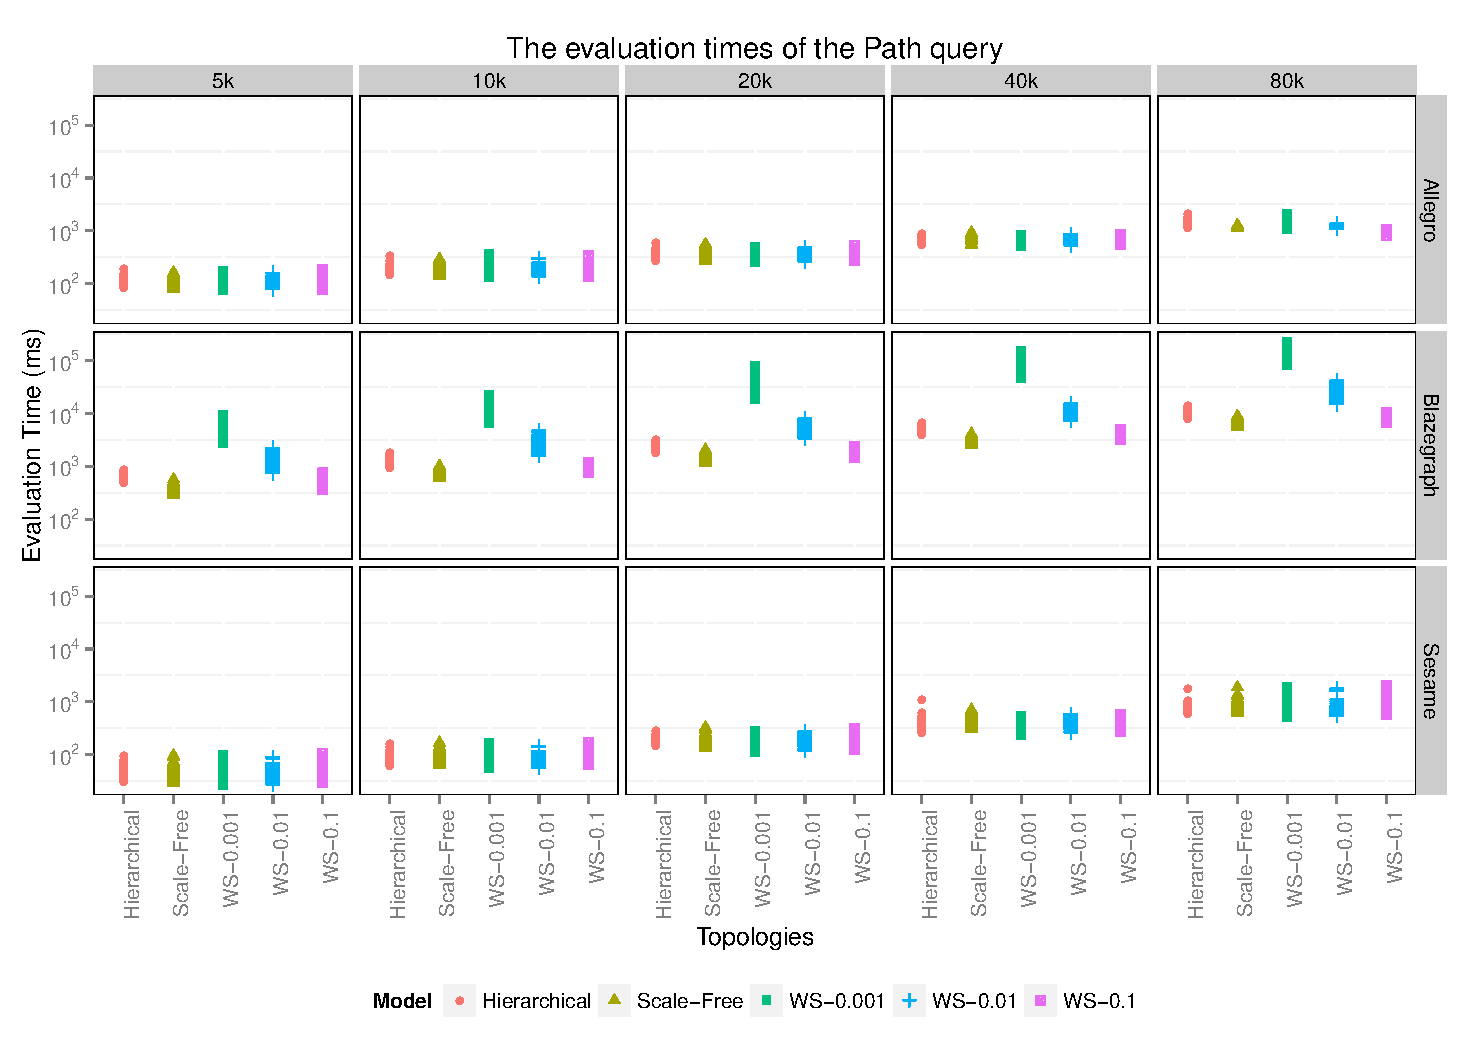
\includegraphics[width=160mm, keepaspectratio]{figures/query1_all.pdf}
	\caption{The measurement results of the Reachability query.}
	\label{fig:query1}
\end{figure}


\label{page:last}
\end{document}
